\documentclass[conference]{IEEEtran}
\IEEEoverridecommandlockouts
\usepackage{cite}
\usepackage{amsmath,amssymb}
\usepackage{graphicx}
\usepackage{booktabs}
\usepackage{makecell}
\usepackage[T1]{fontenc}
\usepackage{textcomp}
\usepackage{url}
\def\UrlBreaks{\do\/\do-\do.\do:}
\input{numbers.tex}
\emergencystretch=1em

\begin{document}
\title{Are Hybrid Ensembles Explained as Faithfully as the Single Model They Replace? Evidence from Eight Healthcare Datasets}

\author{\IEEEauthorblockN{1\textsuperscript{st} Riya Kamboj}
\IEEEauthorblockA{\textit{Department of CSE}\\
\textit{Chandigarh University}\\
Mohali, Punjab-140413, India\\
kzriya004@gmail.com}
\and
\IEEEauthorblockN{2\textsuperscript{nd} Kushalpreet Kaur}
\IEEEauthorblockA{\textit{Department of CSE}\\
\textit{Chandigarh University}\\
Mohali, Punjab-140413, India\\
kushalpreetkaur7@gmail.com}
\and
\IEEEauthorblockN{3\textsuperscript{rd} Ajatray Swagat Bhuyan}
\IEEEauthorblockA{\textit{Department of CSE}\\
\textit{Chandigarh University}\\
Mohali, Punjab-140413, India\\
swagatbhuyan16@gmail.com}}

\maketitle

\begin{abstract}
Clinical prediction studies often combine learners into ensembles and explain them with SHapley Additive exPlanations (SHAP), but rarely test whether these explanations are as faithful as those of the single model the ensemble would replace. We compared a hybrid stacked-voting ensemble with the single model chosen by internal cross-validation on eight public healthcare datasets, using leakage-safe repeated cross-validation, pre-written protocols and a deletion-based faithfulness score computed with two feature-removal methods. Against a pre-specified $\pm$0.02 margin, the ensemble's AUC was equivalent overall (pooled difference \Nauc) and on five datasets, and inconclusive on three. Under marginal feature removal its explanations were less faithful on seven of eight datasets, significantly on three. The pooled decrease (\Nndf) was significant with DerSimonian--Laird pooling but not with the more conservative Hartung--Knapp method (95\% CI \Nndfhk), so it is not definitive. Under conditional removal the difference was smaller and, for untuned models, not significant. Similar patterns held on held-out repetitions, with a second SHAP estimator, with tuned models and without excluding patients. XGBoost alone was explained as faithfully as logistic regression; the ensemble was not. Ensemble explanations should therefore be evaluated, with the removal method stated, rather than assumed faithful.
\end{abstract}


\begin{IEEEkeywords}
explainable AI, ensemble learning, stacking, SHAP, faithfulness, clinical prediction
\end{IEEEkeywords}

\section{Introduction}
Machine-learning models built on routinely collected clinical variables are increasingly proposed for diagnosis and risk stratification \cite{topol}. Ensembles are a frequent choice because combining learners often improves discrimination; a review of disease-prediction studies found stacking to be the most accurate ensemble family in most comparisons where it was used \cite{mahajan}. Because clinical use requires explanations, post-hoc attribution methods such as SHapley Additive exPlanations (SHAP) and LIME are routinely attached to published healthcare ensembles \cite{lundberg2017}.

Attaching an explanation does not show that it is correct. An explanation is \emph{faithful} when the features it ranks highest are the ones that actually drive the model's output. Many explanation methods are still evaluated anecdotally \cite{nauta}, and explainers often disagree on the same prediction \cite{krishna}. A practitioner choosing between an ensemble and a single model therefore has evidence on accuracy, but not on whether the ensemble is explained as faithfully as the simpler alternative.

We study this question for one widely used design, a hybrid stacked-voting ensemble, with analyses specified in dated protocols before they were run and with code and per-fold results that regenerate every number. Our contributions are:
\begin{itemize}
\item A leakage-safe comparison on eight public healthcare datasets between the hybrid ensemble and the single model that internal validation would select: no gain in discrimination, and SHAP explanations that were less faithful under marginal feature removal on seven of eight datasets (significantly on three), with a pooled deficit whose significance depends on the meta-analysis method.
\item Robustness and component analyses: the deficit persists on held-out repetitions, with a second SHAP estimator and with tuned models; it is not a ``linear versus tree'' effect, since XGBoost is explained as faithfully as logistic regression while the ensemble is not.
\item A simulation linking the marginal-removal deficit to correlated features, and a pre-specified held-out test, with a random-grouping placebo, of attribution to clusters of correlated features as a remedy, which helped only where large correlated blocks exist.
\end{itemize}

\section{Related Work}
\subsection{Explained ensembles in healthcare}
Recent conference and journal studies typically pair a stacking or voting ensemble with SHAP or LIME and judge the explanations by clinical plausibility. Divya et al.\ stacked gradient boosting, random forest and logistic regression on the Cleveland data and used SHAP to identify influential features \cite{divya}; Abo-zanona et al.\ combined PCA- and SHAP-guided feature reduction with a tuned stacking ensemble for breast cancer \cite{abozanona}; Ganie et al.\ compared stacking and voting with their base learners on two heart-disease datasets \cite{ganie}. Other studies explain only part of the ensemble or measure a different property: Wolak et al.\ applied SHAP to a CatBoost model rather than to their voting and stacking ensembles \cite{wolak}, Adekoya et al.\ measured the fold-to-fold stability of SHAP rankings computed on one component \cite{adekoya}, Sahin et al.\ reported weak SHAP--LIME agreement for a stacking ensemble \cite{sahin}, and Zarepour-Ahmadabadi et al.\ reported higher local-surrogate fidelity than LIME for a voting ensemble \cite{zarepour}. Neither surrogate fidelity nor explainer agreement shows that the attributed features drive the output \cite{krishna}.

\subsection{Faithfulness metrics and feature removal}
Deletion and insertion curves remove features in order of attributed importance and track the output \cite{petsiuk}; ROAR retrains after removal \cite{hooker}; faithfulness correlation relates attribution mass to the output change for random subsets \cite{bhatt}; ROAD reduces the information leakage and distribution shift that removal introduces \cite{rong}. On clinical tabular data, faithfulness has been evaluated for single models \cite{qureshi,ababneh}; Every removal-based explanation or metric must choose what a removed feature becomes \cite{covert}. Interventional (marginal) replacement is ``true to the model'' but evaluates it on combinations that do not occur in data; conditional replacement is ``true to the data'' but changes what an attribution means \cite{chen,janzing,frye,aas}. Different choices yield different Shapley values \cite{sundararajan,kumar}, and permutation forces models to extrapolate \cite{hooker_mentch}. Group Shapley values were proposed for dependent features \cite{jullum_group}.

Our normalized deletion faithfulness (NDF) is a deletion-curve score that is normalized by the patient's prediction gap and centered on random deletion orders, so that values are comparable across models with different output ranges. ROAD's key idea, imputing removed values in a way that stays close to the data distribution, carries over to tabular data; our conditional $k$-nearest-neighbor operator plays this on-manifold role, and we report it next to the marginal operator because our question is precisely how the removal operator affects the comparison.

\subsection{Positioning}
Table~\ref{tab:rw} contrasts representative studies with ours. We are not aware of a study that compares, on the same patients, the faithfulness of explanations of a fitted heterogeneous ensemble with those of the single model a practitioner would otherwise deploy.

\begin{table}[t]
\caption{Representative studies of explained ensembles and explanation faithfulness on clinical tabular data}
\label{tab:rw}
\centering\scriptsize
\setlength{\tabcolsep}{3pt}
\begin{tabular}{@{}lcccc@{}}
\toprule
Study & Datasets & \makecell{Explains fitted\\ ensemble} & \makecell{Faithfulness\\ measured} & \makecell{Vs.\ selected\\ single model} \\
\midrule
Divya et al.\ \cite{divya} & 1 & Yes & No & No \\
Abo-zanona et al.\ \cite{abozanona} & 1 & Yes & No & No \\
Wolak et al.\ \cite{wolak} & 1 & No (component) & No & No \\
Adekoya et al.\ \cite{adekoya} & 2 & No (component) & No (stability) & No \\
Sahin et al.\ \cite{sahin} & 1 & Yes & No (agreement) & No \\
Zarepour-A.\ et al.\ \cite{zarepour} & 1 & Yes & Surrogate fidelity & No \\
Qureshi et al.\ \cite{qureshi} & 4 & No (single RF) & Yes & No \\
\midrule
This study & 8 & Yes & \makecell{Yes (NDF;\\ FC secondary)} & Yes \\
\bottomrule
\end{tabular}
\end{table}

\section{Methods}
\subsection{Models}
Five components were used: logistic regression (LR), RBF support vector machine (SVM), $k$-nearest neighbors (KNN, $k{=}15$), random forest (RF, 500 trees) and XGBoost \cite{xgboost}, each a pipeline whose imputation and scaling are fitted only on its training data. The \emph{hybrid ensemble} (HE) soft-votes within a linear/kernel/instance group \{LR, SVM, KNN\} and a tree group \{RF, XGB\}, then stacks the two group probabilities with an L2 logistic meta-learner trained on inner 5-fold out-of-fold predictions \cite{wolpert}. The comparator S* is the component with the highest inner out-of-fold AUC on the same training fold, i.e., the single model a practitioner would choose without an ensemble. For robustness we also used soft voting (SV) and logistic stacking (ST) of all five components.

\subsection{Explanations and faithfulness}
Both models are explained on the same patients with permutation SHAP (independent masker, 50 complete-case training rows as background, 500 evaluations, common random numbers per patient). Let $s=\pm1$ be the sign of the predicted class, $F(S)$ the mean prediction after the features in $S$ are replaced by their values in 50 further training rows (\emph{marginal} operator), $[d]$ the set of all $d$ features, $G=s\,(f(x)-F([d]))$ the prediction gap, and $T_k$ the $k$ features with the largest positive signed attributions $s\,\phi_j$, with $K=\min(5, \#\{j: s\phi_j>0\})$. With $D(S)=s\,(f(x)-F(S))/G$, the share of the gap removed by deleting $S$,
\begin{equation}
\mathrm{NDF}(x)=\frac{1}{K}\sum_{k=1}^{K}\Big(D(T_k)-\overline{D}^{\,\mathrm{rand}}_k\Big),
\end{equation}
where $\overline{D}^{\,\mathrm{rand}}_k$ is the mean of $D$ over the first $k$ features of 20 random orderings. NDF is 0 when the top-ranked features remove the prediction no faster than random features and positive when they remove it faster. A \emph{conditional} operator instead takes replacement values from the 20 training rows nearest to $x$ on the kept features.

\emph{Assumptions.} (i) Marginal replacement assumes that features can be changed one at a time; with correlated features it evaluates the model on combinations that do not occur in patients, so NDF then measures faithfulness to the model's behavior under that intervention, not to the data. The conditional operator assumes that 20 nearest neighbors approximate the conditional distribution. Because the two answer different questions \cite{chen}, every faithfulness conclusion below names its operator. (ii) $D$ is a share of the gap and is defined only for $G>0$; it is unstable when $G$ is near zero, so the primary analysis excludes patients with $G<0.05$ for either model. We vary this threshold and also report an exclusion-free version, the absolute deletion faithfulness $\mathrm{ADF}=\mathrm{NDF}\times G$ (prediction drop beyond random deletion, in probability units). (iii) NDF is unbounded: $D$ exceeds 1 when deleting a few features overshoots the all-features-deleted prediction. When $d\le K$ (Mammographic, $d=4$) the $k=d$ term is zero by construction. NDF passed known-answer tests on synthetic models before use (Supplement~S1).

\subsection{Datasets, audit and validation}
Eight binary tasks were used (Table~\ref{tab:data}) \cite{street,antal,detrano,little,uci_repo,uci_cdc,brfss}: three pre-specified datasets (\emph{primary}), four analyzed under a second protocol written before their analysis (\emph{replication}), and a stratified sample of 5{,}000 respondents of the CDC Diabetes Health Indicators survey (\emph{large-sample}). The datasets differ in size, feature types and correlation and come from independent sources; we treat them as separate case studies. Table~\ref{tab:data} gives the audit: label definition, duplicates (removed when they indicate repeated entries, kept when coarse features make identical patients plausible), missing values (imputed inside each training pipeline; explanations used complete cases) and repeated subjects (Parkinsons, folds grouped by person). Each dataset was evaluated with $5\times5$ repeated stratified cross-validation; in every outer fold, 20 complete-case test patients formed the explanation sample.

\subsection{Hypotheses and statistics}
\emph{Confirmatory tests.} H1 (equivalence): $|\Delta\mathrm{AUC}|$ of HE versus S* is below the pre-specified margin of 0.02; tested with two one-sided tests (TOST, 90\% CI within $\pm0.02$) on the 25 fold-level differences, with the corrected repeated cross-validation variance \cite{nadeau}. H2: NDF differs between HE and S* under marginal removal, tested with the same corrected $t$-test and Holm adjustment within each protocol \cite{holm}. The margin was fixed in the protocol; its formal TOST test was added afterwards. Dataset estimates were pooled by DerSimonian--Laird (DL) random effects \cite{dersimonian} with $I^2$ \cite{higgins} and, because eight studies are few, also by the more conservative Hartung--Knapp--Sidik--Jonkman (HKSJ) method \cite{inthout}, with 95\% prediction intervals \cite{riley}.

\subsection{Further analyses}
\emph{Simulation.} 600 patients with ten Gaussian features, an equicorrelated block of four ($\rho\in\{0,0.5,0.9\}$), a linear or non-linear logistic outcome, 3 replicates $\times$ 5 folds; HE versus LR.
\emph{Robustness.} (i) Held-out repetitions 2--5; (ii) KernelSHAP and faithfulness correlation \cite{bhatt} (repetition 1, exploratory); (iii) components tuned by nested grid search (repetition 1); (iv) NDF of each component, SV and ST, and HE versus RF and XGB; (v) exact TreeSHAP; (vi) Monte-Carlo error; (vii) gap thresholds 0.02 and 0.10, ADF, and patients with similar gaps. Analyses (iv)--(vii) and the HKSJ and prediction intervals were added after the primary results were known and are \emph{post hoc}.
\emph{Remedy.} Attributions were summed within clusters of correlated features ($|\rho|\ge0.7$) and NDF computed by deleting whole clusters; found on repetition 1 and tested on repetitions 2--5 against a random-cluster placebo (Supplement S11).


\begin{table*}[t]
\caption{Datasets and audit (UCI repository identifier in parentheses \cite{uci_repo}). Included: sampled explanation patients (500 per dataset) with prediction gap $G\ge0.05$ for both models}
\label{tab:data}
\centering\footnotesize
\setlength{\tabcolsep}{3.2pt}
\begin{tabular}{@{}llrrrlllrr@{}}
\toprule
Dataset & Positive class & $n$ & $d$ & Pos.\,\% & Duplicates & Missing & Repeated subjects & $|\rho|_{\max}$ & Included \\
\midrule
\input{tab_data.tex}
\bottomrule
\end{tabular}\\[2pt]
{\scriptsize $^a$195 recordings of 32 people; outer and inner folds grouped by subject. $^b$Identical records kept: with coarse features they are plausibly different patients. $^c$Stratified sample of 253{,}680 BRFSS 2015 respondents. Missing values were imputed inside each training pipeline; explanation patients and backgrounds were complete cases. $|\rho|_{\max}$: largest Spearman correlation between two features.}
\end{table*}

\begin{table*}[t]
\caption{Primary comparison, HE $-$ S*. Primary columns: means of 25 fold-level differences with 95\% CI; $p$ is Holm-adjusted within each protocol. Robustness columns (secondary or post hoc): conditional removal (25 folds), held-out repetitions 2--5 (20 folds), KernelSHAP and tuned components (repetition 1, 5 folds). $^*p<0.05$, unadjusted}
\label{tab:main}
\centering\footnotesize
\begin{tabular}{@{}lrrrrrrr@{}}
\toprule
 & \multicolumn{3}{c}{Primary (confirmatory)} & \multicolumn{4}{c}{$\Delta$NDF, robustness} \\
\cmidrule(lr){2-4}\cmidrule(lr){5-8}
Dataset & $\Delta$AUC & $\Delta$NDF [95\% CI] & $p$ (Holm) & Conditional & Held-out reps & KernelSHAP & Tuned \\
\midrule
\input{tab_main.tex}
\bottomrule
\end{tabular}\\[2pt]
{\scriptsize $^\dagger$CDC: separate single-dataset protocol, unadjusted. DL: DerSimonian--Laird. HKSJ: Hartung--Knapp--Sidik--Jonkman (computed for the confirmatory outcomes only). Holm-adjusted values are capped at 1.}
\end{table*}

\begin{figure*}[t]
\centering
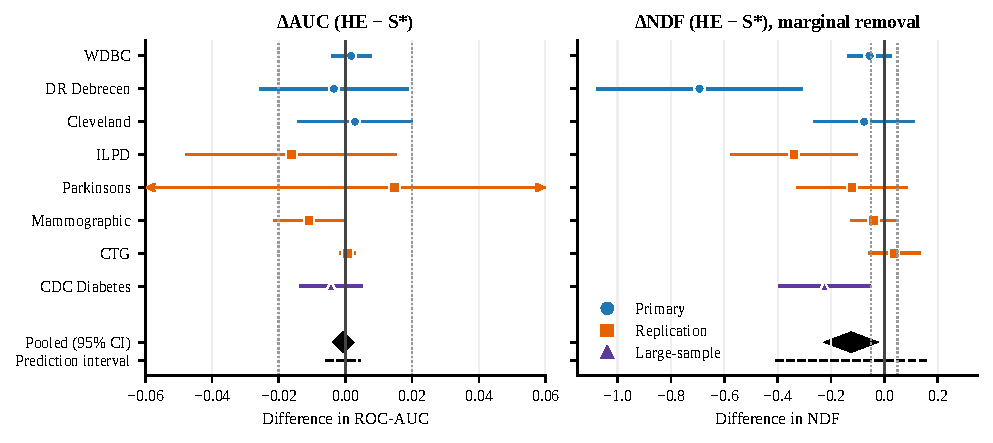
\includegraphics[width=\textwidth]{fig_forest.pdf}
\caption{Per-dataset and pooled differences (HE $-$ S*) with 95\% CI. Left: AUC. Right: NDF under marginal removal. Marker shape and color give the protocol; the diamond is the random-effects pooled estimate and the dashed line the 95\% prediction interval; arrows mark intervals that extend beyond the axis. Dotted lines: pre-specified margins of practical interest ($\pm0.02$ AUC, $\pm0.05$ NDF).}
\label{fig:forest}
\end{figure*}

\section{Results}
\subsection{Discrimination and faithfulness (confirmatory)}
HE did not improve discrimination on any dataset; the pooled AUC difference was \Nauc{} (95\% CI \NaucciL{} to \NaucciH{}; Table~\ref{tab:main}, Fig.~\ref{fig:forest}). Under marginal removal its explanations were less faithful on seven of eight datasets, significantly on diabetic retinopathy (\NpDR, Holm $p\NpDRholm$), liver disease (\NpILPD, Holm $p\NpILPDholm$) and the CDC sample (\NpCDC, $p\NpCDCholm$); no dataset favored HE significantly. The DerSimonian--Laird pooled difference was \Nndf{} (95\% CI \Nndfci; $p\Nndfp$; $I^2=\NndfI\%$), beyond the 0.05 margin of practical interest. Because this method is anti-conservative with few studies, we also computed the HKSJ interval, \Nndfhk{} ($p\Nndfhkp$), and the 95\% prediction interval, \Nndfpi{} (post hoc). The deficit is thus consistent in direction but variable in size, and pooled significance depends on the meta-analysis method.

In the primary analysis the median NDF of included patients was \Nmedhe{} for HE and \Nmeds{} for S*, and HE had the lower NDF for \Nsharelower\% of patients (\NshareDR\% on diabetic retinopathy). In the component analysis (repetition 1), deleting the top-ranked feature removed on average \NtoponeHE\% of HE's prediction gap and \NtoponeS\% of S*'s, versus about \NrandoneS\% for one random feature; deleting the top $K$ removed \NtopKHE\% and \NtopKS\% versus \NrandKS\% for $K$ random features. Shares above 100\% are common (\NoverLR\% of patients for LR): deleting a few top features marginally pushes the prediction past its all-features-deleted value, direct evidence of the off-distribution extrapolation that marginal removal induces \cite{hooker_mentch}. Of \Nnsamp{} sampled patients, \Nexclhe{} (HE) and \Nexcls{} (S*) had $G<0.05$, leaving \Nninc; exclusions were heavy for liver disease and the CDC sample (Supplement S2). With gap thresholds of 0.02 and 0.10 (post hoc), the same three datasets remained significant and the pooled difference was \Nthrtwo{} (HKSJ \Nthrtwohk) and \Nthrten{} (HKSJ \Nthrtenhk). HE's gaps were slightly smaller (median \NGhe{} vs \NGs), but patients with similar gaps showed a similar deficit (\NsimG).

\subsection{Ensembling or non-additive models? (secondary and post hoc)}
The marginal-removal deficit was robust to held-out repetitions (\Nheldout, $p\Nheldoutp$), to KernelSHAP (\Nkernel{} vs \Nperm{} with permutation SHAP on repetition 1) and to tuning (\Ntunndf, $p\Ntunndfp$; Table~\ref{tab:main}). After tuning, S* was SVM, RF or XGB in \Nnlfoldsall{} of \Ntunfolds{} folds (\Nnlfoldsused{} with included patients). With a dataset random intercept, HE's deficit in those folds was \Nnlmix{} (95\% CI \Nnlmixci; $p\Nnlmixp$), smaller and borderline compared with folds where S* was LR (\Nlmix; Table~\ref{tab:robust}). The component analysis is clearer. Median NDF on repetition 1 was \NmedLR{} (LR), \NmedXGB{} (XGB), \NmedSVM{} (SVM), \NmedKNN{} (KNN), \NmedRF{} (RF) and \NmedHE{} (HE); HE was less faithful than XGB (\NHExgb, $p\NHExgbp$) but not than RF (\NHErf), and XGB was as faithful as LR (\NXGBlr). The deficit is therefore not simply ``tree versus linear''. The standard stacking ensemble showed a smaller deficit against S* (\NSTs, $p\NSTsp$) and soft voting a non-significant one (\NSVs). TreeSHAP agreed with permutation SHAP (rank correlation $\ge$\Ntreerho) and Monte-Carlo error was small (Supplement S4--S6). Faithfulness correlation (FC) \cite{bhatt} was lower for HE on average (\Nbhatt, $p\Nbhattp$) but heterogeneous ($I^2=\NbhattI\%$) and, notably, \emph{higher} for HE on diabetic retinopathy (\NFCDR, $p\NFCDRp$), where NDF showed the largest deficit. FC rewards a linear relation between summed attribution and output change over random subsets, which spreading credit over near-duplicate counts can raise, whereas NDF rewards removing the prediction quickly with the top-ranked features; the two metrics therefore capture different properties (Supplement S7).

\begin{table}[t]
\caption{Robustness of the deficit (secondary and post hoc): pooled $\Delta$NDF over eight datasets, repetition 1}
\label{tab:robust}
\centering\scriptsize
\resizebox{\columnwidth}{!}{\begin{tabular}{@{}lrrrr@{}}
\toprule
 & \multicolumn{2}{c}{Marginal removal} & \multicolumn{2}{c}{Conditional} \\
\cmidrule(lr){2-3}\cmidrule(lr){4-5}
Comparison & $\Delta$NDF [95\% CI] & $p$ & $\Delta$NDF & $p$ \\
\midrule
\input{tab_robust.tex}
\bottomrule
\end{tabular}}\\[2pt]
{\scriptsize SV, ST: soft-voting and stacking ensembles of all five components. Comparison rows: DerSimonian--Laird. Tuned rows: fold means with a dataset random intercept.}
\end{table}

\subsection{Removal operator and simulation (secondary)}
For untuned models, the pooled difference under conditional removal was smaller, \Nknn{} ($p\Nknnp$); on diabetic retinopathy it shrank from \NpDR{} to \NpDRknn. With tuned components, however, a substantial conditional deficit remained (fold means with a dataset random intercept: \Ntunallmixk, $p\Ntunallmixkp$, versus \Ntunallmix{} marginal; \Nnlmixk{} when S* was non-linear), and HE was less faithful than RF only under conditional removal (Table~\ref{tab:robust}). The operator therefore modulates the deficit for untuned models but does not explain it in general; we did not investigate why tuning changes this. In the simulation (Supplement S9), the marginal-removal deficit of HE relative to LR grew with within-block correlation under a linear outcome (\NsimLzero, \NsimLhalf{} and \NsimLnine{} at $\rho=0$, 0.5, 0.9) but stayed near zero under conditional removal (interaction \Nsimint, SE \Nsimintse; $p\Nsimintp$).

\subsection{Correlation-aware remedy}
In the exploratory discovery analysis, attributing to clusters of correlated features narrowed the deficit. The pre-specified test on held-out repetitions (Table~\ref{tab:remedy}) confirmed this where large correlated blocks exist: on diabetic retinopathy the deficit fell from \NdfeatDR{} to \NdgrpDR{} (reduction \NRDR, $p\NRDRp$), and correlation clusters outperformed random clusters of the same sizes (\NPLDR, $p\NPLDRp$); reductions were also significant on liver disease (\NRILPD) and WDBC (\NRWDBC). The pre-specified pooled hypothesis was not supported (pooled reduction \NpoolR, $p\NpoolRp$): clustering enlarged the gap on cardiotocography (\NRCTG), and over all datasets correlation clusters did no better than random ones (\NpoolPL, $p\NpoolPLp$). A pre-specified non-additivity explanation for the remaining deficit was also not supported (Supplement S8).

\begin{table}[t]
\caption{Remedy: $\Delta$NDF (HE $-$ S*) with feature- and cluster-level attribution. Discovery: repetition 1. Confirmation: held-out repetitions 2--5}
\label{tab:remedy}
\centering\scriptsize
\setlength{\tabcolsep}{2.5pt}
\begin{tabular}{@{}lrrrrr@{}}
\toprule
 & Discovery & \multicolumn{4}{c}{Confirmation (pre-specified)} \\
\cmidrule(lr){2-2}\cmidrule(lr){3-6}
Dataset & Reduction & $\Delta$NDF feature & $\Delta$NDF cluster & Reduction $R$ & Placebo \\
\midrule
\input{tab_remedy.tex}
\bottomrule
\end{tabular}\\[2pt]
{\scriptsize Reduction = cluster $-$ feature $\Delta$NDF; Placebo = reduction with correlation clusters minus reduction with random clusters of the same sizes. $^*p<0.05$.}
\end{table}

\section{Discussion}
For the hybrid stacked-voting ensemble studied here, the evidence supports three conclusions of different strength. First, the ensemble added no discrimination: its AUC was equivalent to the selected model's overall and on five datasets, and inconclusive, not inferior, on three. Second, \emph{under marginal feature removal} its SHAP explanations were less faithful: the effect was consistent in direction (seven of eight datasets, significant on three, never significantly reversed under NDF) and robust to the checks above, but varied in size, and the pooled decrease was significant only with the less conservative meta-analysis method. Third, the conclusion depends on the removal method: for untuned models the difference under conditional removal was small and not significant, whereas with tuned models a conditional deficit remained. Statements about faithfulness should therefore always name the removal method; ours do not establish that ensemble explanations are less faithful under every definition.

The component analysis refines the interpretation. The deficit is not a generic ``linear versus tree'' effect: XGBoost was explained as faithfully as logistic regression, whereas random forest and nearest neighbors were not, and HE was explained about as faithfully as random forest. We hypothesize that averaging step-like and piecewise-constant components spreads attribution over correlated features and makes the ensemble respond less predictably to off-manifold inputs \cite{hooker_mentch,chen}; the one mechanism we tested directly, non-additivity, was not supported.

\emph{Clinical relevance.} On diabetic retinopathy, HE's explanation was less faithful than the selected model's for \NshareDR\% of patients: a clinician reading HE's top-ranked feature would, on average, be pointed to a feature that accounts for less of the risk score. Studies proposing clinical ensembles should therefore compare against the selected single model, explain the fitted ensemble and state the removal method.

\emph{Limitations and future work.} We studied one hybrid architecture, binary tasks and public datasets of at most 5{,}000 patients, analyzed as case studies; Parkinsons has only 32 subjects; exclusions by the gap threshold were heavy for two datasets, although an exclusion-free measure gave the same pattern; logistic regression was the selected comparator in most untuned folds; and no clinicians evaluated the explanations. This paper covers the SHAP faithfulness part of a broader explanation-reliability framework. LIME explanations, their stability under small input changes, and agreement between explainers are left for future work, as are external validation and larger clinical cohorts.

\section{Conclusion}
On eight healthcare datasets, a hybrid stacked-voting ensemble matched the discrimination of the internally selected single model within a pre-specified margin overall, while its SHAP explanations were less faithful under marginal feature removal on seven datasets, significantly on three. The pooled decrease was significant with DerSimonian--Laird pooling but not with the more conservative Hartung--Knapp method, and it was smaller under conditional removal; it should be read as a consistent but not definitive deficit. Explanation faithfulness should be reported alongside accuracy, with the removal method stated, when ensembles are proposed for clinical use. The supplement (S1--S13), protocols, code and per-fold outputs are at \url{https://github.com/RiyaKamboj/xai-hybrid-ensemble-faithfulness}.



\begin{thebibliography}{99}
\input{refs.tex}
\end{thebibliography}
\end{document}
